\documentclass[12pt,a4paper]{report}
\usepackage[top=1in,bottom=1in,left=1.3in,right=0.8in]{geometry}

\usepackage{listings}
\usepackage{color}
\usepackage{verbatim}

\usepackage[pdftex,%
	pdfauthor=Akash{ }Shende,%
	pdftitle={myproject},%
	pdfsubject={project report},%
	pdfkeywords={project},%
	pdfproducer=Akash{ }Shende,%
	pdfcreator=pdflatex]{hyperref}

\usepackage{fancyhdr}
\usepackage{pgfgantt}
\usepackage{rotating}
\usepackage{tikz-uml}
\usepackage[fleqn]{amsmath}
\usepackage{chngcntr}
\usepackage{tikz-er2}
\usepackage{multicol}
\usepackage{tikz}
\usepackage{caption}
\usepackage{subcaption}
\usepackage{times}
\usepackage{algorithmicx}
\usepackage{framed}
\usepackage{array}
\usetikzlibrary{arrows,shapes,trees,positioning}
\usetikzlibrary{shadows}


%setting for code snippets
\definecolor{dkgreen}{rgb}{0,0.6,0}
\definecolor{gray}{rgb}{0.5,0.5,0.5}
\definecolor{mauve}{rgb}{0.58,0,0.82}
 
\lstset{ %
  language=Python,                % the language of the code
  basicstyle=\footnotesize\ttfamily,           % the size of the fonts that are used for the code
  numbers=left,                   % where to put the line-numbers
  numberstyle=\scriptsize\color{gray},  % the style that is used for the line-numbers
  stepnumber=1,                   % each line is numbered
  numbersep=5pt,                  % how far the line-numbers are from the code
  backgroundcolor=\color{white},      % choose the background color. You must add \usepackage{color}
  showspaces=false,               % show spaces adding particular underscores
  showstringspaces=false,         % underline spaces within strings
  showtabs=false,                 % show tabs within strings adding particular underscores
  frame=shadowbox,                   % adds a frame around the code
  rulecolor=\color{black},        % if not set, the frame-color may be changed on line-breaks within not-black text (e.g. commens (green here))
  tabsize=4,                      % sets default tabsize to 2 spaces
  captionpos=b,                   % sets the caption-position to bottom
  breaklines=true,                % sets automatic line breaking
  breakatwhitespace=false,        % sets if automatic breaks should only happen at whitespace
  title=\lstname,                   % show the filename of files included with \lstinputlisting;
                                  % also try caption instead of title
  keywordstyle=\color{blue},          % keyword style
  commentstyle=\color{dkgreen},       % comment style
  stringstyle=\color{mauve},         % string literal style
  escapeinside={\%*}{*)},            % if you want to add a comment within your code
  morekeywords={*,self,__init__,None,cv2,np,cv,float32,array,len,list...}               % if you want to add more keywords to the set
}





%set line spacing
\linespread{1.3}

\hypersetup{pdfborder={0 0 0}}

\counterwithout{figure}{chapter}
\counterwithout{table}{chapter}

%document starts here
\begin{document}

\pagenumbering{Roman}
\thispagestyle{empty}
\linespread{1.3}

%Acknowledgement is written in abstract environement so it appears in middle of page.
% Remember: Dont left a half page blank.It looks ugly.Instead left equal space from top and bottom side.
\renewcommand{\abstractname}{\sc \Large{Acknowledgement}}
\begin{abstract}

\noindent It was a great experience to develop {\bf{``Your project title''}}. Many people helped us for this project,those must be appreciated.\\[0.3cm]
\noindent We are profoundly grateful to {\bf Prof.guide name} for her expert guidance and continuous encouragement throughout to see that this project achieves its target since its commencement to its completion.\\[0.3cm]
\noindent We would like to express deepest appreciation towards {\bf principal , Principal college city, Prof.HOD name, Head Of Department name and Prof.coordinator name (Project Coordinator)} whose invaluable guidance supported us in completing this project. At last we must express our sincere heartfelt gratitude to all the staff members of Department name who helped us directly or indirectly during this course of work.\\[0.3cm]


\hfill
{\bf
\begin{tabular}{l}
Student name1\\
Student name2\\
Student name3
\end{tabular}
}
\end{abstract}


\linespread{1}
%\rfoot{\footnotesize{Page \thepage}}
%\lfoot{\footnotesize{Department of Computer Engineering, JSCOE Pune}}
%\cfoot{}
%\cleardoublepage
%\phantomsection
\addcontentsline{toc}{chapter}{\numberline{}Abstract}
%\addtocontents{toc}{\protect\settocdepth{-1}}
\renewcommand{\abstractname}{\Large Abstract}
\begin{abstract}
\setcounter{page}{1}
\thispagestyle{plain}
\normalsize{}
\noindent YOUR ABSTRACT \\[0.3cm]
\smallskip
\noindent \textbf{Keywords} some keywords, other keywords
\end{abstract}

{\protect\thispagestyle{plain}}

\pagestyle{empty}
\addtocontents{toc}{\protect\thispagestyle{empty}}
\renewcommand\contentsname{Table Of Contents}
\tableofcontents
\newpage%
\setcounter{page}{5}
\phantomsection
\addcontentsline{toc}{chapter}{\numberline{}List of Figures}
\addtocontents{lof}{\protect\thispagestyle{plain}}
\listoffigures%{\protect\thispagestyle{plain}}
\cleardoublepage
\setcounter{page}{7}
\addcontentsline{toc}{chapter}{\numberline{}List of Tables}
\listoftables{\protect\thispagestyle{plain}}
\clearpage


\pagestyle{fancy}
\fancyhead{} % clear all header fields
\setlength{\headheight}{14.50pt}
\renewcommand{\footrulewidth}{1pt}
\renewcommand{\chaptermark}{
\rhead}
\lhead{\chaptername{} \thechapter}

\fancypagestyle{plain}{%
  \fancyhf{}\fancyfoot[R]{\footnotesize{Page \thepage}}%
\lfoot{\footnotesize{Department of Computer Engineering, JSCOE Pune}} %NOTE: this footer is for the page where Chapter start,place your college name 
  \renewcommand{\headrulewidth}{0pt}}

\rfoot{\footnotesize{Page \thepage}}
\lfoot{\footnotesize{Department of Computer Engineering, JSCOE Pune}}%NOTE: this footer is for all pages,place your college name 
\cfoot{}


\pagestyle{fancy}
\newpage

\pagenumbering{arabic}
\chapter{Introduction}
\noindent{\Huge I}ntro to your project. Remember, first line of paragraph should not be indented\\
\indent From immediate next paragraph, use indent.

\section{Motivation}
\noindent ABC DEF...

\section{Background}
\noindent Why you implemented your system, describe in informal words.

\section{The Concept}
Your project concept in informal, concise words\\
Example of bullet list
\begin{itemize}\itemsep-5pt
\item item1
\item item2
\item item3
\end{itemize} 

 %completed
\chapter{Literature Survey}


\section{paper 1}
adding cross references (see Figure~\ref{fig:3dtracking}) 

%adding image
\begin{figure}[ht!]
\centering
\includegraphics[width=60mm]{file_name.jpg}
\caption[caption in LOF]{caption appear below the image}
\label{fig:reflabel}
\end{figure}

 %completed 
\chapter{Proposed System}
YOUR sections, according to your project
 %95%
\chapter{Research Methodology}

Adding equation, Example:\\
\noindent RGB to HSV conversion formula is as follows\cite{dip}.\\
\textit{R, G, B are values of pixel}
\begin{align}
R'=R/255 \nonumber \\
G'=G/255\nonumber \\
B'=B/255\nonumber
\end{align}
\begin{eqnarray}
Cmax=max(R', G', B')\nonumber \\
Cmin=min(R', G', B')\nonumber 
\end{eqnarray}
\begin{eqnarray}
\Delta=Cmax-Cmin\nonumber
\end{eqnarray}
\textit{Hue calculation}
\begin{eqnarray}
H=\begin{cases}
	60^\circ \times \left(\frac{G'-B'}{\Delta} \mod 6\right) \text{if Cmax=R'}\\
	60^\circ \times \left(\frac{B'-R'}{\Delta} + 2 \right) \text{if Cmax=G'}\\
	60^\circ \times \left(\frac{R'-G'}{\Delta} + 4 \right) \text{if Cmax=B'}
\end{cases}
\end{eqnarray}
\clearpage
\noindent \textit{Saturation calculation}

\begin{eqnarray}
S=\begin{cases}
	0 & \text{if}\Delta \text{=0} \\
	\frac{\Delta}{Cmax} & \text{if}\Delta \neq \text{ 0}
\end{cases}
\end{eqnarray}
\textit{Value calculation}
\begin{eqnarray}
\large{V=Cmax}
\end{eqnarray}

 %0%
\chapter{Designing}


Contains, SRS, UML diagrams, ER,DFDs\\

example of table\\

\subsubsection{Hardware requirements}

\begin{table}[ht!]
{\bf
\begin{tabular}{l|l}
\hline
\textit{Processor} & Intel{\textsuperscript{\textregistered}} Core{\textsuperscript{\texttrademark}}2 Quad,Q8300, 2.50GHz \\
\textit{Memory} & 2048MB\\
\textit{Camera} & Logitech c270 (3MP, 800x600 RGB @ 20 fps)\\
\textit{Display device} & Dell 22" TFT-LCD Monitor\\
\textit{Other} & othes\\ \hline
\end{tabular}
}
\end{table}

\newpage
\subsection{System Architecture}
an example of Block diagram

\begin{figure}[ht!]
\centering
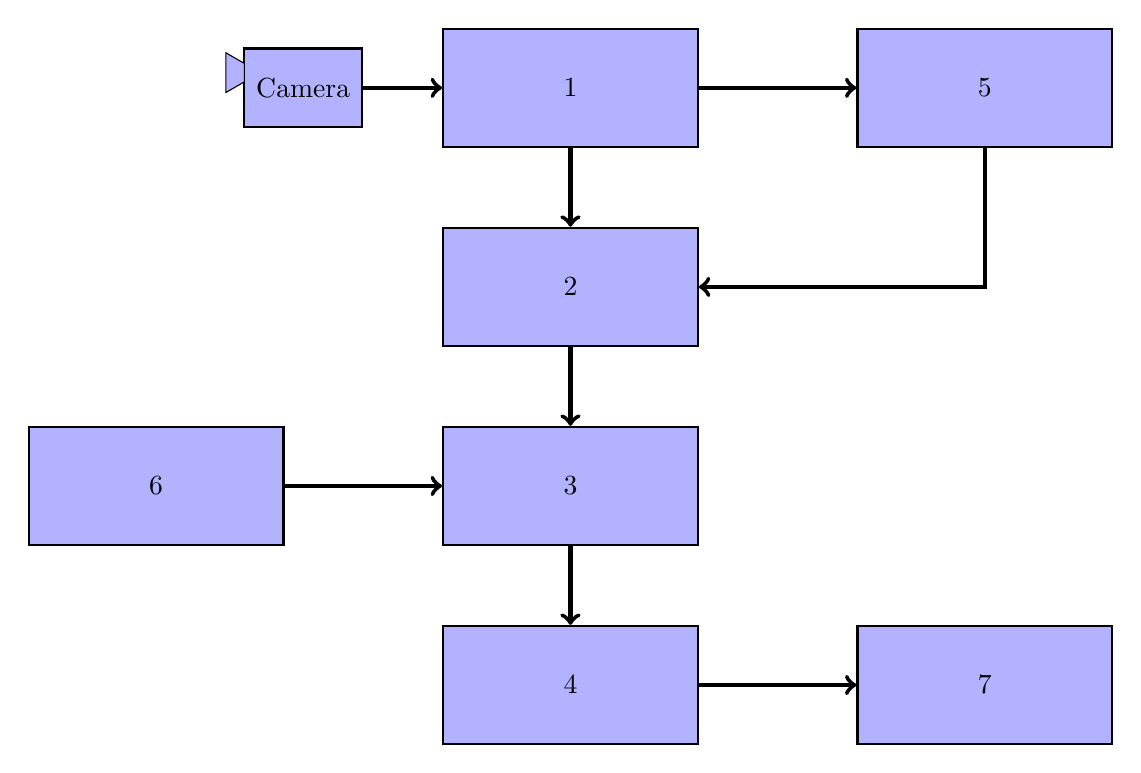
\begin{tikzpicture}[mystyle/.style={draw,rectangle,fill=blue!30,thick,minimum width=3cm,minimum height=1.5cm}]

\node[mystyle,text width=3cm,align=center](a){1};
\node[mystyle,text width=3cm,align=center](b)[below=of a]{2};
\node[mystyle,text width=3cm,align=center](c)[below=of b]{3};
\node[mystyle,text width=3cm,align=center](d)[below=of c]{4};

\node[mystyle,node distance=2cm,text width=3cm,align=center](e)[right=of a]{5};
\node[mystyle,node distance=2cm,text width=3cm,align=center](f)[left=of c]{6};

\node[mystyle,node distance=2cm,text width=3cm,align=center](g)[right=of d]{7};
\node[mystyle,minimum width=1.5cm,minimum height=1cm](h)[left=of a]{Camera};
\node[style={draw,trapezium,fill=blue!30,rotate=-90,above=4cm},node distance=0.1cm](z)[left=of h]{};


\draw[->,ultra thick](a)--(b);
\draw[->,ultra thick](b)--(c);
\draw[->,ultra thick](c)--(d);
\draw[->,ultra thick](f)--(c);
\draw[->,ultra thick](a)--(e);
\draw[->,ultra thick](e)|-(b);
\draw[->,ultra thick](d)--(g);
\draw[->,ultra thick](h)--(a);

\end{tikzpicture}
\caption{caption}
\end{figure}

\clearpage

\section{ER Diagram, example of ER daigram}
\begin{figure}[ht!]
\tikzstyle{every entity}=[top color=white,bottom color=blue!30,draw=blue!30!black!100, drop shadow,node distance=1cm,minimum width=3cm, minimum height=1cm]
\tikzstyle{every relationship}=[top color=white,bottom color=red!30, draw=black!100,node distance=1cm,minimum width=1.5cm, minimum height=0.5cm]
\tikzstyle{every attribute}=[top color=white,bottom color=yellow!40,draw=red, drop shadow,node distance=0.7cm,text width=2cm]

\scalebox{0.78}{
\begin{tikzpicture}

\node[entity](cam){entity1};
\node[relationship,text width=1.5cm](info)[right=of cam]{rel1} edge[<-,line width=2](cam);
\node[relationship,text width=1.5cm](provides)[below=of info]{rel2} edge[<-,line width=2](cam);
\node[entity](sys)[right=of info]{entity2} edge[<-,line width=2](info);
\node[relationship,text width=2cm](norm)[below=of sys]{rel} edge[<-,line width=2](sys);
\node[entity](vid)[below=of norm]{entity3} edge[<-,line width=2](provides) edge[<-,line width=2](norm) ;

\node[relationship,text width=1.5cm](proces)[below =of vid]{rel} edge[<-,line width=2](vid);

\node[entity](bg)[left=of proces]{entity} edge[<-,line width=2](proces);

\node[entity](replace)[left=of bg]{entity} edge[<-,line width=2](bg);
\node[entity,node distance=2cm](out)[above=of replace]{entity} edge[<-,line width=2](replace);
\node[relationship](rel_replce)[below=of replace]{rel} edge[<-,line width=2](replace);

\node[entity](tshirt)[right=of rel_replce]{entity} edge [<-,line width=2](rel_replce);

%attributes started
%Camera
\node[attribute][left=of cam]{attribut} edge[line width=2,draw=blue] (cam);
\node[attribute][above left=of cam]{attribute} edge[line width=2,draw=blue] (cam);

%System
\node[attribute][right=of sys]{attribute} edge[line width=2,draw=blue](sys);

%video
\node[attribute][right=of vid]{attribute} edge[line width=2,draw=blue](vid);
\node[attribute][right=of vid]{attribute} edge[line width=2,draw=blue](vid);

%replace
\node[attribute][left=of replace]{attribute} edge[line width=2,draw=blue](replace);
\node[attribute][above left=of replace] {attribute} edge[line width=2,draw=blue](replace);

%tshirt
\node[attribute][below right=of tshirt]{attribute} edge[line width=2,draw=blue](tshirt);
\node[attribute][below=of tshirt]{attribute} edge[line width=2,draw=blue](tshirt);

%removeBG
\node[attribute,node distance=0.5cm][below left=of bg]{attribute} edge[line width=2,draw=blue](bg);
\node[attribute,node distance=2.5cm][below right=of bg]{attribute} edge[line width=2,draw=blue](bg);
\node[attribute][below=of bg]{attribute} edge[line width=2,draw=blue](bg);


%output
\node[attribute][above left=of out]{attribute} edge[line width=2,draw=blue](out);
\node[attribute][above =of out]{attribute} edge[line width=2,draw=blue](out);
\node[attribute][right=of out]{attribute} edge[line width=2,draw=blue](out);

%arrows
%\draw[link](cam)-|(info);
\end{tikzpicture}
}
\caption{caption}
\end{figure}

\clearpage

\section{Data Flow Diagram,example}
\subsection{Context level}
\begin{figure}[ht!]
\centering
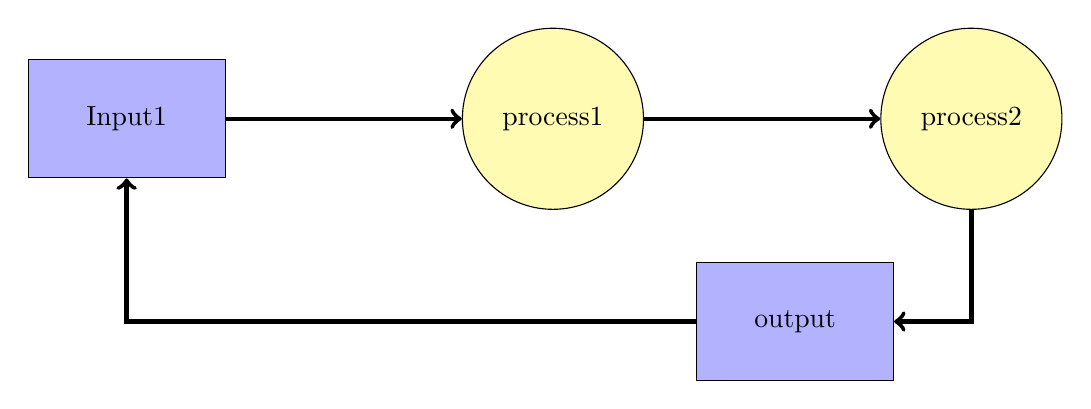
\begin{tikzpicture}

%\begin{umlstate}{0}
%\end{umlstate}

%\filldraw[fill=yellow!30,label=0] (0,0) circle (1cm);
\node[style={draw,circle,fill=yellow!30,minimum height=2.3cm}](a){process1};
\node[style={draw,circle,fill=yellow!30,minimum height=2.3cm,node distance=3cm}](b)[right=of a]{process2};

\node[style={draw,rectangle,minimum width=2.5cm,minimum height=1.5cm,fill=blue!30,node distance=3cm}](c)[left=of a]{Input1};
\node[style={draw,rectangle,minimum width=2.5cm,minimum height=1.5cm,fill=blue!30}](d)[below right=of a]{output};

\draw[ultra thick][->](c)--(a);
\draw[ultra thick][->](a)--(b);
\draw[ultra thick][->](b)|-(d);
\draw[ultra thick][->](d)-|(c);
\end{tikzpicture}
\caption{DFD: Context level}
\end{figure}

\clearpage


\section{UML Modelling}
\begin{comment}
sequence 
1] use case [done
2] class [done
3] state [done
4] sequence [doen
5] activity
6] deployment [done
7] component [done
\end{comment}

\subsection{Usecase diagram}

\begin{figure}[ht!]
\begin{tikzpicture}
\begin{umlsystem}[x=3,y=0]{Usecase}

\umlactor[x=-4,y=-2]{Customer}
\umlactor[x=5,y=-3]{System}
\umlusecase[x=0,y=-1,name=cap_vid,fill=green!50]{usecase}
\umlusecase[x=0,y=-2,name=proc,fill=green!50]{usecase}
\umlusecase[x=0,y=-3,name=temp_sel,fill=green!50]{usecase}
\umlusecase[x=0,y=-4,name=out,fill=green!50]{usecase}
\umlassoc{Customer}{cap_vid}
\umlassoc{Customer}{temp_sel}
\umlassoc{System}{proc}
\umlassoc{System}{out}
\end{umlsystem}
\end{tikzpicture}
\caption{Usecase diagram}
\end{figure}
\clearpage

\begin{comment}
\subsection{Class Diagram}
\begin{figure}[ht!]
\begin{tikzpicture}
\begin{umlpackage}{vdr}

\umlclass[x=7,y=-1,width=3cm]{Video}{
	\-- capture:cvcapture\\
	\-- frame:array

}{
	+getCapture():cvcapture\\
	+outFrame():array\\
	+imagePlanes(image:array):array
}

\umlemptyclass[type=interface,x=11,y=-4]{vdr}
{
	+color:int\\
}{}

\umldep[anchor1=west,anchor2=25,geometry=--,stereo=uses]{RemoveBG}{NormalizedRGB}

\umldep[geometry=--,anchor1=north,]{RemoveBG}{Video}

\umlreal[angle1=0,angle2=north,anchor1=30,anchor2=north,geometry=-|,pos=.5]{MainUI}{vdr}

\umlreal[geometry=-|]{Replace}{vdr}
\umlaggreg[geometry=--,anchor1=-160]{Video}{NormalizedRGB}
\umlassoc{Tshirt}{Replace}
\umlassoc[geometry=|-,anchor1=130,anchor2=-30]{RemoveBG}{Tshirt}
\umlassoc[geometry=-|-,anchor1=-45,anchor2=-140]{MainUI}{Replace}
\end{umlpackage}
\end{tikzpicture}
\caption{Class diagram}
\end{figure}
\clearpage
\end{comment}
\subsection{State transition digram}

\begin{figure}[ht!]
\centering
\scalebox{0.85}{

\begin{tikzpicture}
\umlstateinitial[name=start]

\begin{umlstate}[name=cam,y=-3.5]{state1}
\end{umlstate}

\begin{umlstate}[name=video,y=-7.5]{state2}
\end{umlstate}

\begin{umlstate}[name=extract,y=-11.5]{state3}
\end{umlstate}

\begin{umlstate}[name=project,y=-11.5,x=6]{state4}
\end{umlstate}


\begin{umlstate}[name=templates,y=-15.5]{state5}
\end{umlstate}

\begin{umlstate}[name=display,y=-15.5,x=6]{state6}
\end{umlstate}

\begin{umlstate}[name=update,y=-19.5]{state7}
\end{umlstate}

\begin{umlstate}[name=next,y=-19.5,x=6]{state8}
\end{umlstate}

\umlstatefinal[name=stop,y=-22]

\umltrans[arg=Ready]{start}{cam}
\umltrans[arg=captures]{cam}{video}
\umltrans[arg=Extract]{video}{extract}
\umltrans[arg=project]{extract}{project}
\umltrans[arg=GUI]{project}{display}
\umltrans[arg=selection]{display}{templates}
\umltrans{templates}{update}
\umltrans{update}{next}
\umlHVHtrans[anchor2=east,arm2=2cm,arm1=2cm,anchor1=east,arg=Yes]{next}{project}
\umlVHtrans[arg=No]{next}{stop}

\end{tikzpicture}
}


\caption{State diagram}
\end{figure}
\clearpage

\subsection{Sequence diagram}

%classes: Camera, Background subtraction, Detection, Replace, Out
\begin{figure}[ht!]
\centering
\begin{sideways}
\scalebox{1}
{
\begin{tikzpicture}
\tikzumlset{font=\scriptsize}

\begin{umlseqdiag}
\umlobject[class=Main]{main}
\umlobject[class=Camera]{cam}
%\umlobject[class=Video,x=2.5]{video}
\umlcreatecall[class=Video, draw obj=green!70!black,fill obj=green!30]{main}{video}
\umlcreatecall[class=Remove, draw obj=green!70!black,fill obj=green!30]{video}{remove}
%\umlcreatecall[class=Tshirt]{main}{tshirt}
%\umlcrearecall[class=Replace]{tshirt}{replace}
 %x=5
\umlobject[class=Tshirt]{tshirt}%,x=7.6
\umlcreatecall[class=Replace, draw obj=green!70!black,fill obj=green!30,]{tshirt}{replace}
%\umlobject[class=Remove]{remove}%,x=10.5
%\umlobject[class=Replace]{replace}%,x=14


\begin{umlcallself}[op={provide GUI}]{main}
\end{umlcallself}
\begin{umlcall}[op={get\_frame()},return=frame]{video}{cam}
\end{umlcall}

\begin{umlcall}[op={background}]{cam}{remove}
\end{umlcall}

\begin{umlcall}[op={request o/p()},return=video]{main}{video}
	\begin{umlcall}[op={normalized video}]{video}{remove}
		\begin{umlcall}[op={processed}]{remove}{replace}
			\begin{umlcall}[op={replacing}]{replace}{tshirt}
				\begin{umlcall}[op={final o/p}]{tshirt}{main}
					\begin{umlcallself}[op={display o/p}]{main}
					\end{umlcallself}
				\end{umlcall}
			\end{umlcall}
		\end{umlcall}
	\end{umlcall}
\end{umlcall}
\end{umlseqdiag}
\end{tikzpicture}
}

\end{sideways}
\caption{Sequence diagram}
\end{figure}
\clearpage



\subsection{Component Diagram}
\begin{figure}[ht!]
\centering
\scalebox{0.80}{
\begin{tikzpicture}
\begin{umlcomponent}{Virtual dressing room}

\begin{umlcomponent}{MainUI}
\end{umlcomponent}

\begin{umlcomponent}[x=6]{Camera}
\end{umlcomponent}

\begin{umlcomponent}[x=12,y=-2]{Video}
\end{umlcomponent}

\begin{umlcomponent}[x=0,y=-4]{Screen}
\end{umlcomponent}

\begin{umlcomponent}[x=5,y=-7]{Remove Back}
\end{umlcomponent}

\begin{umlcomponent}[x=5.5,y=-3.5]{vdr}
\end{umlcomponent}
%\umlrequiredinterface[interface=hue, distance=2cm,width=0.5cm]{vdr}


\begin{umlcomponent}[x=11,y=-6]{Replace}
\end{umlcomponent}

\begin{umlcomponent}[x=10,y=-10]{Tshirt}
\end{umlcomponent}

\umlassemblyconnector[interface=hue]{Replace}{vdr}
\umlassemblyconnector[interface=hue]{MainUI}{vdr}
\umlassemblyconnector{Remove Back}{Video}
\umlHVassemblyconnector{Screen}{Replace}
\draw[draw=black,dashed][->](MainUI)|-(Video);
\draw[draw=black,dashed][<-](Camera)-|(Video);
\draw[draw=black,dashed][->](Tshirt)--(Remove Back);
\draw[draw=black,dashed][<-](Tshirt)--(Replace);
\draw[draw=black,dashed][<-](Screen)--(MainUI);

\end{umlcomponent}
\end{tikzpicture}
}
\caption{Component diagram}
\end{figure}

 %50

\chapter{Implementation}

example of adding code snippet
\lstinputlisting[language=xml]{ui.xml}
This Glade XML file clearly shows different widget included in GUI. For example, from line number 38 to 45 describes the main windows properties, its title, position on screen,etc.
\section{Analysis}
\subsubsection{Mathematical model}

Let S be the system that takes input image and updates it with the selected template.\\
S=\{$I,O,F,Sc,Fc$\}\\
where,\\
\indent I=Input\\
\indent O=Ouput\\
\indent T=Templates\\
\indent Sc=Success case\\
\indent Fc=Failure case\\

Dm=\{$Dm1,Dm2,...,Dm_{n}|Dm_{i}$ is template applying function\} \\
Dg=\{$Dg1,Dg2,...,Dg_{n}|Dg_{i}$ is updated image representation\} \\
\indent Where,$Dg_{i}$=\{U\} U=\{$U1,U2,...,Un$\} Where, U is updated frames.\\

\noindent $F1:$ template updation()\\
$F1:$(Tm) Dgc\\
$Tm$ selected template\\
$Dgc$ updated image\\

\begin{figure}[ht!]
\centering
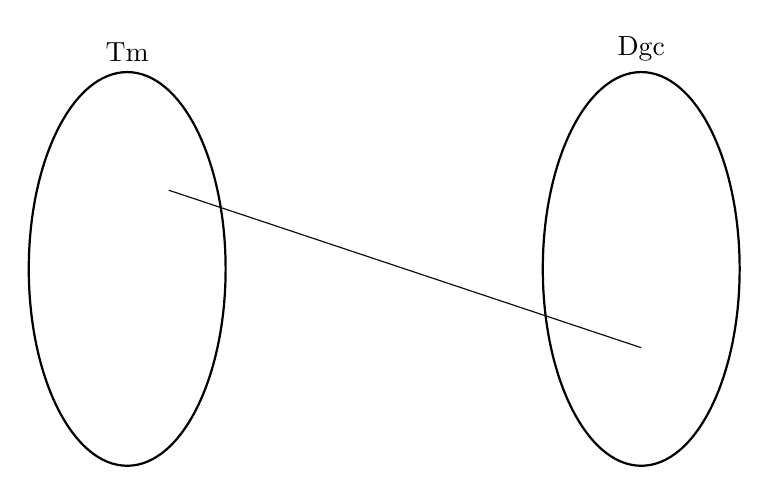
\begin{tikzpicture}

\node[ellipse,minimum height=5cm,draw=black,thick,minimum width=2.5cm,name=cir1,label=Dgc]{};

\node[ellipse,minimum height=5cm,draw=black,thick,minimum width=2.5cm,node distance=4cm,name=cir2,label=Tm][left=of cir1]{};

\coordinate (a) at (0,-1);
\coordinate (b) at (-6,1);
%\fill[blue](a) circle (3pt);
%\fill[blue](b) circle (3pt);
\draw (a)--(b);
\end{tikzpicture}
\caption{Venn diagram}
\end{figure}

\noindent SuccessCases: Sc=\{$Sc1\wedge Sc2 \wedge Sc3 \wedge Sc4$\}\\
$Sc1$ Input frame generated correctly\\
$Sc2$ Template selected correctly\\
$Sc3$ Template applied successfully\\
$Sc4$ Output frame generated successfully\\

\noindent Failure Cases: Fc=\{$Fc1,Fc2,Fc3, Fc4$\}, O=$\phi$\\
$Fc1$ Camera error\\
$Fc2$ template not selected successfully\\
$Fc3$ errors while applying template.\\
$Fc4$ output file not displayed .
\clearpage
\section{Results}

\clearpage
 %0
\chapter{Testing}

\section{Unit testing}

\section{integration testing}


\section{Acceptance testing}




%\begingroup{
%\setlength\parskip{-20pt}
\chapter{Scheduling}
%}

Example of Gantt chart
\begin{figure}[ht!]
\centering
\begin{sideways} %rotate figure
\scalebox{1}{
\begin{ganttchart}[hgrid=false, vgrid={*{13}{blue,dashed},*1{red,very thick}}, x unit=.7cm, y unit chart=.7cm, 
bar/.style={fill=green, rounded corners=3pt,draw=none},bar height=.3,
group/.style={fill=green},
incomplete/.style={fill=red},
canvas/.style={draw=blue,thick},
title/.style={draw=blue,thick},
grid/.style={draw=none}]{22}
\gantttitle{Project Schedule}{22}
\\
\gantttitle{Jun-12}{2}
\gantttitle{Jul}{2}
\gantttitle{Aug}{2}
\gantttitle{Sep}{2}
\gantttitle{Oct}{2}
\gantttitle{Nov}{2}
\gantttitle{Dec}{2}
\gantttitle{Jan-13}{2}
\gantttitle{Feb}{2}
\gantttitle{Mar}{2}
\gantttitle{Apr}{2}
\\
\ganttgroup[progress=100]{\small Designing \& Modelling}{1}{10}\\*[0pt]
\ganttbar[name=info,progress=100]{\bf \scriptsize Info gathering}{1}{3.7}\\
\ganttlinkedbar[progress=100]{\bf \scriptsize  Outline diagrams}{2.7}{3}\\
\ganttlinkedbar[progress=100]{\bf \scriptsize Math. model}{3}{4.3} \ganttnewline[thick,blue]

\ganttbar[progress=100]{\bf \scriptsize Deciding functions}{3.3}{5.5}\\
\ganttlinkedbar[name=func_depend,progress=100]{\bf \scriptsize Functional dependency}{5.5}{7}\\
\ganttmilestone[name=submit,progress=100]{\bf \scriptsize Partial Report Submission}{10} \ganttnewline[thick,blue]
\ganttlink{func_depend}{submit}

\ganttgroup[progress=90]{Coding}{12}{17}\\*[0cm]
\ganttbar[progress=100]{\bf \scriptsize setup}{12.7}{13.5}\\
\ganttbar[progress=98]{\bf \scriptsize module1}{13.3}{13.8}\\
\ganttlinkedbar[progress=95]{\bf \scriptsize modul2}{13.8}{14}\\
\ganttlinkedbar[progress=93]{\bf \scriptsize module3}{14}{15.5}\\
\ganttbar[name=interface,progress=99]{\bf \scriptsize module4}{13.8}{16.5}\\
\ganttmilestone[name=finish_code]{\bf \scriptsize Finalized Coding}{17} \ganttnewline[thick,blue]
\ganttlink{interface}{finish_code}

\ganttgroup[progress=92]{Testing \& Deployment}{14}{22}\\*[0cm]
\ganttbar[progress=85]{\bf \scriptsize Testing}{14}{20}\\
\ganttlinkedbar[progress=100]{\bf \scriptsize Project Demo}{20}{20.2}\\
\ganttbar[name=report,progress=100]{\bf \scriptsize Final Report}{20}{21.5}\\*[0.5cm]
\ganttmilestone[name=end]{\bf \scriptsize Final Submission}{21.7}
\ganttlink{report}{end}
%\ganttlinkedbar{info}{3}{7} \ganttnewline
%\ganttmilestone{Milestone}{7} \ganttnewline
%\ganttbar{Final Task}{8}{12}
%\ganttlink{elem2}{elem3}
%\ganttlink{elem3}{elem4}
\end{ganttchart}
}
\end{sideways}
\caption[Project planner]{Project planner\\ \scriptsize{Note: Designing \& modelling phase includes information gathering also}}
\label{fig:gantt}
\end{figure}
\clearpage
\section{Work Breakdown Structure}

\tikzset{
every node/.style={draw,text width=2cm},
style1/.style= {rectangle, rounded corners=2pt, thin,align=center,fill=green!30,text width=5cm},
style2/.style= {rectangle, rounded corners=6pt, thin,align=center,fill=green!60,yshift=-2cm,text width=2.5cm},
style3/.style= {rectangle,thin,align=left,fill=blue!20,yshift=-1cm,text width=2.5cm},
style4/.style= {draw=white,thin,align=center,fill=white}
}


\begin{figure}[ht!]
\begin{tikzpicture}[
remember picture,
level 1/.style={sibling distance=35mm},
edge from parent/.style={->,draw,thick},
>=latex]

% the initial tree ("root" and "text nodes")
\node[style1] {1 main}
child {node[style2] (c1) {1.1 subwork}}
child {node[style2] (c2) {1.2 subwork}}
child {node[style2] (c3) {1.3 subwork}}
child {node[style2] (c4) {1.4 subwork}};

% the nodes below each of the "text" nodes
\node [style3,below of = c1,xshift=15pt,yshift=-1cm] (c11) {1.1.1 \\ subwork};
\node [style3,below of = c11] (c12) {1.1.2\\subwork};
\node [style3,below of = c12] (c13) {1.1.3\\ subwork};
\node [style3,below of = c13] (c14) {1.1.4\\subwork};

\node [style3,below of = c2,xshift=15pt,yshift=-1cm] (c21) {1.2.1\\subwork};
\node [style3,below of = c21] (c22) {1.2.2\\subwork};
\node [style3,below of = c22] (c23) {1.2.3\\subwork};

\node [style3,below of = c3,xshift=15pt,yshift=-1cm] (c31) {1.3.1\\subwork};
\node [style3,below of = c31] (c32) {1.3.2\\subwork};
\node [style3,below of = c32] (c33) {1.3.3\\subwork};
\node [style3,below of = c33] (c34) {1.3.4\\subwork};

\node [style3,below of = c4,xshift=15pt,yshift=-1cm] (c41) {1.4.1\\subwork};
\node [style3,below of = c41] (c42) {1.4.2\\subwork};
\node [style3,below of = c42] (c43) {1.4.3\\subwork};
\node [style3,below of = c43] (c44) {1.4.4\\subwork};

\node[style4] at (6,0) {Level1};
\node[style4] at (8.5,-3.5) {Level2};
\node[style4] at (8.5,-8) {Level3};

% lines from each "text" node to every one of its "children"
\foreach \value in {1,2,3,4}
  \draw[thick,->] (c1.195) |- (c1\value.west);

\foreach \value in {1,...,3}
  \draw[thick,->] (c2.195) |- (c2\value.west);

\foreach \value in {1,...,4}
  \draw[thick,->] (c3.195) |- (c3\value.west);

\foreach \value in {1,...,4}
 \draw[thick,->] (c4.195) |- (c4\value.west);
\end{tikzpicture}
\caption{Work Breakdown Structure}
\label{fig:wbs}
\end{figure}



\renewcommand{\thechapter}{}{}
\renewcommand{\chaptername}{}{}
\cleardoublepage
\phantomsection
\addcontentsline{toc}{chapter}{Advantages}
\chapter*{Advantages} %skip to add toc, adding it manually


advantages
 %advantages
%\input{future.tex} %future scope
%\input{conclusion.tex} %conclusion
%\input{ref.tex}
\appendix
\chapter{Appendix 1}
\clearpage

\chapter{Appendix 2}




\end{document}
